\documentclass[fleqn,10pt,lineno]{wlpeerj}

\usepackage{siunitx}
\usepackage{algorithm}
\usepackage{algorithmic}
\usepackage{multirow}
\usepackage{url}
\usepackage{hyperref}

\title{Predicci\'on de Bus Bunching mediante Se\~nales de Alerta Temprana en un Digital Twin de Transporte P\'ublico}

\author[1]{Carlos Stiven Mora Hoyos}
\author[1]{Juan Felipe Rodr\'iguez Galindo}
\author[1]{Octavio Jos\'e Salcedo Parra}
\affil[1]{Facultad de Ingenier\'ia, Maestr\'ia en Ciencias de la Informaci\'on y las Comunicaciones, Universidad Distrital Francisco Jos\'e de Caldas, Bogot\'a, Colombia}
\corrauthor[1]{Carlos Stiven Mora Hoyos}{csmorah@udistrital.edu.co}
% Author emails: csmorah@udistrital.edu.co, juafrodriguezg@udistrital.edu.co, osalcedo@udistrital.edu.co

\begin{abstract}
El bus bunching es una anomal\'ia operacional estoc\'astica que deteriora severamente la confiabilidad de corredores de transporte p\'ublico de alta frecuencia. Aunque la integraci\'on de datos General Transit Feed Specification Realtime (GTFS-RT) en arquitecturas de Digital Twin (DT) ha sido ampliamente adoptada, los modelos predictivos existentes frecuentemente exhiben altas tasas de falsos positivos debido al ruido de se\~nales urbanas, o no proporcionan suficiente tiempo de anticipaci\'on para la intervenci\'on operacional. Este art\'iculo propone un marco algor\'itmico emp\'irico de Se\~nales de Alerta Temprana (Early Warning Signal, EWS) centrado en la eficiencia computacional y la validaci\'on secuencial. Utilizando un conjunto de datos de $\approx$100 millones de registros brutos de Localizaci\'on Autom\'atica de Veh\'iculos (Automatic Vehicle Location, AVL) del sistema San Francisco Muni (enero--marzo de 2026)---estrictamente depurados a 3.365.545 observaciones con lag v\'alido para el modelado secuencial---demostramos que una ventana secuencial multi-parada ($n{-}3$) enriquecida con razones de headway, retraso diferencial del bus l\'ider y contexto de programaci\'on filtra eficazmente el ruido transitorio. Mientras que la literatura previa frecuentemente reporta m\'etricas infladas (F1 $>$ 0,80) debido a fuga de datos espacio-temporal y umbrales est\'aticos de anomal\'ia, establecemos un r\'egimen riguroso de evaluaci\'on utilizando partici\'on temporal estricta (hold-out) y definiciones din\'amicas de bunching ($h_{obs} < 0,25 \cdot h_{sch}$). Nuestros resultados muestran que un modelo de gradient boosting LightGBM con caracter\'isticas de raz\'on informadas por la f\'isica alcanza una precisi\'on operacional de 0,93 (IC 95\%: [0,92; 0,93]) y un F1-score de 0,55 (IC 95\%: [0,55; 0,56]) para predecir bunching inminente dentro de un horizonte de 3 paradas. De manera crucial, identificamos la raz\'on de headway ($h_{obs}/h_{sch}$) y el diferencial relativo de retraso entre buses consecutivos como las se\~nales precursoras primarias, confirmando el mecanismo en cascada de la propagaci\'on del bunching. Adicionalmente, reportamos una latencia de inferencia de 1,89 milisegundos por registro, lo que permite el monitoreo en tiempo real a escala regional. Estos resultados de filtrado espacio-temporal y modelado de transici\'on de estados informan la gesti\'on proactiva del transporte en entornos de tr\'afico mixto y establecen la base para estrategias de control en sistemas BRT.
\end{abstract}

\begin{document}

\flushbottom
\maketitle
\thispagestyle{empty}

\section{Introducci\'on}

El bus bunching constituye una de las principales fallas operacionales en redes de transporte p\'ublico de alta frecuencia \citep{1,21}. Este fen\'omeno ocurre cuando la separaci\'on temporal entre veh\'iculos consecutivos en la misma l\'inea---denominada headway---disminuye progresivamente hasta que dos o m\'as buses viajan en convoy. \citet{1} formaliz\'o el mecanismo causal: cuando un bus acumula un retraso marginal en una parada, la demanda de pasajeros en las paradas subsiguientes aumenta, amplificando el retraso original; simult\'aneamente, el veh\'iculo siguiente encuentra menos pasajeros y acelera su recorrido, reduciendo la brecha entre ambos. \citet{2} demostr\'o que esta retroalimentaci\'on positiva es inherente a las l\'ineas de alta frecuencia y crece exponencialmente sin mecanismos de control activo. Como consecuencia, el servicio se degrada en forma de tiempos de espera excesivos para los pasajeros y distribuci\'on desigual de la carga entre veh\'iculos \citep{3}.

En la pr\'actica, la mayor\'ia de las agencias de transporte gestionan sus flotas utilizando horarios est\'aticos definidos bajo el est\'andar General Transit Feed Specification (GTFS). Estos horarios establecen tiempos de llegada planificados a cada parada, pero carecen de capacidad predictiva para anticipar eventos de bunching. \citet{21} se\~nalan que la detecci\'on operacional del bunching es predominantemente reactiva: los centros de control identifican el evento solo despu\'es de que ya se ha manifestado, limitando las posibilidades de intervenci\'on preventiva.

En paralelo, las arquitecturas de Digital Twin (DT) han emergido como un paradigma para el monitoreo y control proactivo de flotas \citep{5,6}. Un DT de transporte construye una r\'eplica virtual de la flota f\'isica a partir de datos de Localizaci\'on Autom\'atica de Veh\'iculos (AVL) transmitidos v\'ia GTFS Realtime (GTFS-RT) \citep{7}. No obstante, la disponibilidad de telemetr\'ia en tiempo real no resuelve por s\'i sola el problema de predicci\'on. Los marcos predictivos existentes enfrentan dos limitaciones documentadas: altas tasas de falsos positivos originadas por la varianza estoc\'astica del tr\'afico urbano (ciclos sem\'aforicos, estacionamiento en doble fila, congesti\'on localizada), y sobrecarga computacional que impide latencias compatibles con la intervenci\'on operacional en tiempo real \citep{8,9}.

Este art\'iculo propone un m\'etodo para predecir el bus bunching \textit{antes} de que ocurra, con suficiente tiempo de anticipaci\'on para que los operadores intervengan. Mientras que los m\'etodos convencionales analizan lo que ocurre en una \'unica parada \citep{8}, la literatura reciente ha demostrado que la incorporaci\'on de informaci\'on de m\'ultiples paradas precedentes mejora la capacidad de distinguir perturbaciones transitorias de tendencias genuinas de deterioro \citep{3,15}. Siguiendo esta l\'inea, nuestro enfoque examina la trayectoria del bus en las tres paradas precedentes ($n{-}3$) junto con caracter\'isticas de raz\'on informadas por la f\'isica---raz\'on de headway ($h_{obs}/h_{sch}$), raz\'on de retraso y retraso diferencial del bus l\'ider---que codifican el mecanismo en cascada de la propagaci\'on del bunching. Para la clasificaci\'on, exponemos las limitaciones de los modelos lineales en datos altamente desbalanceados y con alto ruido, y empleamos un modelo de gradient boosting LightGBM con ponderaci\'on de desbalance de clases. Adem\'as, criticamos estudios previos que reportan F1 superior a 0,80 demostrando c\'omo los umbrales fijos (por ejemplo, brechas fijas de 120s) y las particiones aleatorias 80/20 introducen fuga de datos severa e inflan artificialmente la clase positiva. Al aplicar estrictamente partici\'on temporal (hold-out) y la definici\'on din\'amica te\'oricamente robusta de bunching ($h_{obs} < 0,25 \cdot h_{sch}$), alcanzamos predicciones operacionalmente confiables (Precision = 0,93, F1 = 0,56) dentro de un horizonte de 3 paradas. Adicionalmente, incorporamos predicci\'on conformal---una t\'ecnica estad\'istica que, en lugar de emitir alertas binarias, adjunta a cada predicci\'on un conjunto de etiquetas posibles con una garant\'ia calibrada de cobertura (por ejemplo, 90\%), permitiendo al operador distinguir alertas de alta confianza de casos ambiguos. La validaci\'on se realiza sobre un conjunto de datos del San Francisco Municipal Railway (SF Muni) procesado con DuckDB \citep{14} como motor anal\'itico embebido.

Concretamente, las contribuciones de este trabajo son:
\begin{itemize}
  \item Un espacio de caracter\'isticas informado por la f\'isica ($n{-}3$, 24 caracter\'isticas) que incorpora razones de headway ($h_{obs}/h_{sch}$), retraso diferencial del bus l\'ider, frecuencia programada y progresi\'on espacial para capturar el mecanismo en cascada de la propagaci\'on del bunching.
  \item Una cr\'itica metodol\'ogica que establece que la validaci\'on cruzada est\'andar (por ejemplo, 80/20) y los umbrales temporales fijos inducen fuga de datos espacial y temporal, conduciendo a m\'etricas EWS artificialmente infladas ($F1 > 0,80$).
  \item Una evaluaci\'on rigurosa con partici\'on temporal (hold-out) que demuestra que bajo la definici\'on din\'amica de bunching ($h_{obs} < 0,25 \cdot h_{sch}$), un modelo de gradient boosting LightGBM alcanza precisi\'on operacionalmente confiable ($0,93$) y F1-score ($0,56$).
  \item Una capa de predicci\'on conformal que adjunta conjuntos de confianza calibrados a cada alerta, de modo que los operadores puedan identificar alertas de alta certeza frente a situaciones ambiguas que requieren verificaci\'on.
  \item Un benchmark computacional que demuestra latencia de pocos milisegundos utilizando DuckDB, viable para despliegue en arquitecturas Digital Twin Edge-Cloud de baja latencia.
  \item C\'odigo y datos abiertos para reproducibilidad completa.
\end{itemize}

El art\'iculo est\'a organizado de la siguiente manera: la Secci\'on~\ref{sec:related} revisa el estado del arte. La Secci\'on~\ref{sec:methodology} describe la arquitectura del sistema y la formulaci\'on matem\'atica. La Secci\'on~\ref{sec:experiments} detalla la configuraci\'on experimental. La Secci\'on~\ref{sec:results} presenta los resultados. La Secci\'on~\ref{sec:discussion} discute las implicaciones y limitaciones. La Secci\'on~\ref{sec:futurework} describe las direcciones futuras, y la Secci\'on~\ref{sec:conclusion} concluye.

\section{Trabajo Relacionado}
\label{sec:related}

Para construir un marco EWS robusto, este estudio integra literatura de cuatro dominios: din\'amica de headway, arquitecturas de ingesti\'on de datos, modelado predictivo con datos desbalanceados y marcos de Digital Twin.

\subsection{Din\'amica de Headway y la F\'isica del Bus Bunching}

La inestabilidad de las l\'ineas de alta frecuencia fue formalizada matem\'aticamente por \citet{1}, quien demostr\'o que la varianza del headway crece exponencialmente sin control activo. \citet{2} extendi\'o esta l\'inea proponiendo estrategias autocoordinadas basadas en headway que reemplazan los horarios est\'aticos con ecualizaci\'on din\'amica del headway. Estos trabajos fundacionales establecen que la distancia relativa entre buses consecutivos (headway) es una m\'etrica de estabilidad superior comparada con la adherencia al horario (retraso). Estudios recientes de \citet{3} y \citet{8} modelan el bunching como un problema de transici\'on de estados, utilizando datos AVL y GTFS-RT para rastrear c\'omo las perturbaciones locales se propagan espacialmente a trav\'es de la red urbana. \citet{10} demostr\'o que los tiempos de retenci\'on basados en headways cuasi-regulares reducen las penalizaciones por bunching hasta en un 45\%, siempre que el mecanismo de detecci\'on sea preciso.

\subsection{Datos GTFS Realtime y Arquitecturas de Ingesti\'on}

La proliferaci\'on de datos abiertos de transporte ha habilitado an\'alisis operacionales a gran escala. \citet{11} propusieron metodolog\'ias para extraer m\'etricas de desempe\~no a partir de componentes GTFS-RT y clasificar retrasos sistem\'aticos versus estoc\'asticos. Sin embargo, el gran volumen de datos AVL impone desaf\'ios significativos de procesamiento \citep{12}. Las bases de datos relacionales tradicionales orientadas a filas (RDBMS) introducen latencia sustancial en el c\'omputo de funciones de ventana secuenciales (por ejemplo, operaciones \texttt{LAG} sobre millones de filas) \citep{13}. Para abordar esto, estudios recientes promueven bases de datos anal\'iticas embebidas orientadas a columnas. \citet{14} introdujeron DuckDB como una base de datos en proceso altamente optimizada, capaz de ejecutar consultas anal\'iticas complejas sin sobrecarga de red. La aplicaci\'on de estas arquitecturas a la predicci\'on de retrasos a escala urbana ha sido validada por \citet{15}, enfatizando la necesidad de ingenier\'ia de caracter\'isticas multi-resoluci\'on con latencia m\'inima.

\subsection{Aprendizaje Autom\'atico para Datos de Transporte Desbalanceados}

Predecir el bus bunching es inherentemente un problema de clasificaci\'on desbalanceada, ya que los eventos de bunching constituyen la clase minoritaria (t\'ipicamente del 5\% al 10\% de las observaciones) bajo operaci\'on nominal \citep{16}. Los clasificadores est\'andar basados en umbrales o los modelos optimizados por precisi\'on global no capturan adecuadamente la clase minoritaria, generando sub-predicci\'on severa de anomal\'ias. \citet{17} demostraron que los enfoques de manejo de desbalance centrados en F1-Score y el \'area bajo la curva Precision-Recall (PR-AUC) son obligatorios para evitar sesgo de estimaci\'on en modelos de transporte. Adem\'as, \citet{18} mostraron que abordar el desbalance es cr\'itico en la predicci\'on estoc\'astica de anomal\'ias de transporte. Aunque los modelos de aprendizaje profundo como el BAT-transformer \citep{19} alcanzan alta precisi\'on en la predicci\'on de tiempos de llegada, operan como ``cajas negras'' y requieren altos recursos computacionales. En contraste, la regresi\'on log\'istica optimizada proporciona interpretabilidad para los despachadores mientras mantiene poder predictivo competitivo cuando las caracter\'isticas espacio-temporales est\'an adecuadamente dise\~nadas \citep{20}. \citet{21} ofrecen una revisi\'on integral indicando que, a pesar de la popularidad del aprendizaje profundo, los modelos lineales con espacios de caracter\'isticas robustos tienden a ser m\'as pr\'acticos para el despliegue en tiempo real.

\subsection{Sistemas de Alerta Temprana en Transporte P\'ublico}

Los Sistemas de Alerta Temprana (Early Warning Systems, EWS) constituyen una clase espec\'ifica de mecanismos predictivos orientados a se\~nalar el inicio inminente de una anomal\'ia antes de que se manifieste completamente, distingui\'endose de los detectores reactivos que operan \textit{a posteriori} \citep{4}. En el dominio del transporte p\'ublico, la detecci\'on de anomal\'ias operacionales ha sido hist\'oricamente abordada mediante gr\'aficos de control estad\'istico (CUSUM), modelos adaptativos de desviaci\'on de headway con umbrales, y m\'etodos de procesos gaussianos sobre series temporales de puntualidad \citep{8}. Estos enfoques generan alertas cuando una m\'etrica ya ha excedido un umbral predefinido, implicando tiempos de anticipaci\'on insuficientes para acciones de mitigaci\'on preventiva.

Los clasificadores de anomal\'ias---incluyendo m\'etodos no supervisados (Isolation Forests), detectores semi-supervisados (One-Class SVM) y modelos supervisados de transici\'on de estados---han emergido como alternativas predictivas, habilitando la detecci\'on de firmas de deterioro antes del colapso observable \citep{3}. No obstante, aplicarlos en corredores urbanos de tr\'afico mixto enfrenta el desaf\'io del severo desbalance de clases (eventos an\'omalos $\ll$ 10\% de las observaciones nominales) y la alta varianza ex\'ogena de los corredores compartidos \citep{16}. Los modelos de predicci\'on profunda (transformers \citep{19}, redes con celdas de memoria) alcanzan alta precisi\'on en tiempos de llegada pero operan como cajas negras con latencias incompatibles con el monitoreo DT en tiempo real \citep{30}.

El marco propuesto en este art\'iculo se posiciona en la intersecci\'on de EWS predictivos y arquitectura DT de baja latencia: adoptamos un formalismo de predicci\'on de transici\'on de estados ($B_{n-1}=0 \rightarrow \tilde{B}_n=1$, formalizado en la Secci\'on~\ref{sec:methodology}) para eliminar el sesgo de persistencia presente en los detectores reactivos, y envolvemos las alertas con predicci\'on conformal para proporcionar garant\'ias probabil\'isticas calibradas en lugar de alarmas binarias no cuantificadas.

\subsection{Arquitecturas de Digital Twin y Computaci\'on en el Borde}

Un Digital Twin de transporte integra telemetr\'ia en tiempo real con modelos predictivos para construir una r\'eplica virtual de la flota f\'isica \citep{22,23}. \citet{24} describen requisitos estructurales para DTs de transporte p\'ublico sostenible, destacando capacidades de simulaci\'on ``what-if''. Sin embargo, estas capacidades dependen de la generaci\'on de EWS con baja latencia. \citet{25} proponen arquitecturas DT para Sistemas Inteligentes de Transporte (ITS) que demandan eficiencia computacional estricta para la sincronizaci\'on continua entre estados f\'isicos y virtuales. En consecuencia, los paradigmas de computaci\'on en el borde (edge computing) se identifican como habilitadores clave de DTs de baja latencia \citep{26}. Al procesar datos cerca de la fuente o utilizar herramientas anal\'iticas en proceso altamente eficientes, las agencias pueden evitar los cuellos de botella de las arquitecturas centralizadas en la nube \citep{27}. Esta arquitectura h\'ibrida Edge-Cloud es consistente con los requisitos de resiliencia y seguridad observados en despliegues de Digital Twin habilitados por IoT \citep{31}.

\section{Arquitectura del Sistema y Metodolog\'ia}
\label{sec:methodology}

\subsection{Pipeline de Datos del Digital Twin}

El sistema propuesto funciona como la capa predictiva de un Digital Twin de transporte. Su objetivo es recibir datos de posici\'on de buses en tiempo real, procesarlos y generar alertas antes de que ocurra el bunching. El pipeline consiste en tres etapas secuenciales: (1) ingesti\'on de datos GTFS-RT, (2) transformaci\'on y limpieza, y (3) inferencia predictiva.

Un requisito central del sistema es que la inferencia sea suficientemente r\'apida para operar en tiempo real. Por lo tanto, en lugar de utilizar bases de datos convencionales como PostgreSQL, optamos por DuckDB \citep{14}, un motor anal\'itico embebido que se ejecuta dentro del mismo proceso de la aplicaci\'on. DuckDB procesa datos en formato columnar y en bloques, habilitando la ejecuci\'on de operaciones de ventana (como comparar la posici\'on actual de un bus con sus posiciones previas) con eficiencia muy superior a la de los sistemas cliente-servidor tradicionales. Comparado con herramientas como Pandas, DuckDB adicionalmente ofrece ejecuci\'on paralela y gesti\'on eficiente de memoria, haci\'endolo especialmente adecuado para procesar los flujos masivos de datos AVL caracter\'isticos de GTFS-RT. Esta arquitectura alcanza una extracci\'on de caracter\'isticas de baja latencia adecuada para la operaci\'on en tiempo real.

Un paso cr\'itico en la transformaci\'on es la resoluci\'on del orden temporal a partir de los flujos AVL brutos. Dado que los registros \texttt{StopTimeUpdate} de GTFS-RT proporcionan tiempos previstos de llegada y salida por viaje y parada, el pipeline selecciona la marca temporal de salida cuando est\'a disponible (recurriendo a la de llegada en su defecto) y la convierte a segundos del d\'ia para un c\'omputo secuencial consistente. El motor anal\'itico DuckDB aplica entonces funciones de ventana (\texttt{LAG}, \texttt{LEAD}) particionadas por ruta, fecha de servicio y veh\'iculo para computar headways inter-vehiculares y variables de estado secuenciales. Las observaciones con contexto de lag inv\'alido (por ejemplo, el primer veh\'iculo del d\'ia en una parada, o brechas que superan los 7.200 segundos entre veh\'iculos consecutivos) se excluyen de la inferencia para evitar que valores de caracter\'isticas espurios contaminen la ventana secuencial.

\subsection{Formulaci\'on Matem\'atica de los Estados del Sistema}

Para formalizar cu\'ando un bus est\'a en bunching, definimos dos m\'etricas complementarias. La primera es el retraso ($D$), que mide cu\'anto se desv\'ia un bus de su horario programado. Sean $T_{obs}(i, v_k)$ y $T_{sch}(i, v_k)$ el tiempo de llegada observado y programado del veh\'iculo $v_k$ a la parada $i$, respectivamente:
\begin{equation}
  D(i, v_k) = T_{obs}(i, v_k) - T_{sch}(i, v_k)
\end{equation}

Sin embargo, el retraso por s\'i solo no indica bunching: un bus puede tener 5 minutos de retraso y operar establemente si el bus siguiente tambi\'en tiene un retraso similar. Lo que realmente determina la estabilidad del sistema es la distancia temporal entre buses consecutivos, conocida como headway ($h$). Definimos el headway observado $h_{obs}$ entre el veh\'iculo $v_2$ y su predecesor $v_1$ en la misma ruta como:
\begin{equation}
  h_{obs}(i) = T_{obs}(i, v_2) - T_{obs}(i, v_1)
\end{equation}
An\'alogamente, el headway programado es:
\begin{equation}
  h_{sch}(i) = T_{sch}(i, v_2) - T_{sch}(i, v_1)
\end{equation}

Con estas dos m\'etricas, podemos definir formalmente cu\'ando un bus est\'a en bunching. Siguiendo est\'andares de la industria \citep{1,10}, declaramos bunching cuando el headway observado cae por debajo del 25\% del headway programado---es decir, cuando la distancia temporal entre buses se ha reducido a menos de un cuarto del valor planificado:
\begin{equation}
  B_i =
  \begin{cases}
    1, & \text{si } h_{obs}(i) < 0,25 \cdot h_{sch}(i) \\
    0, & \text{en caso contrario}
  \end{cases}
\end{equation}

Para predecir el bunching dentro de un horizonte de 3 paradas en lugar de en una sola parada, definimos el objetivo agregado:
\begin{equation}
  \tilde{B}_n = \max(B_n, B_{n+1}, B_{n+2})
\end{equation}
El modelo predictivo utiliza $\tilde{B}_n$ como variable objetivo: dada la observaci\'on actual en la parada $n$, predecir si ocurrir\'a bunching en cualquiera de las siguientes tres paradas. El filtro de transici\'on de estados retiene solo las observaciones donde $B_{n-1}=0$ (el bus no estaba en bunching en la parada inmediatamente anterior), eliminando los casos de persistencia trivialmente predecibles y enfoc\'andose exclusivamente en las transiciones de inicio operacionalmente relevantes.

\subsection{Ingenier\'ia de Caracter\'isticas Espacio-Temporales (Ventana $n{-}3$)}

Una vez definido qu\'e significa bunching, la pregunta clave es: \textquestiondown podemos predecirlo antes de que ocurra? Para este fin, en lugar de observar solo la parada inmediatamente anterior, examinamos el comportamiento del bus en las tres paradas precedentes ($n{-}1, n{-}2, n{-}3$). Este enfoque de ventana multi-parada permite distinguir entre una fluctuaci\'on transitoria (un sem\'aforo en rojo) y una tendencia genuina de deterioro.

El vector de caracter\'isticas $X \in \mathbb{R}^{24}$ se organiza en cuatro grupos. El primer grupo captura el estado absoluto (retraso $D$ y headway observado $h_{obs}$ en cada parada precedente) y la tasa de cambio entre paradas consecutivas:
\begin{equation}
  \Delta D_j = D(n-j) - D(n-j-1), \quad \Delta H_j = h_{obs}(n-j) - h_{obs}(n-j-1) \quad \text{para } j \in \{1, 2\}
\end{equation}

El segundo grupo introduce \textit{caracter\'isticas de raz\'on informadas por la f\'isica} que normalizan los valores absolutos por el headway programado, codificando la definici\'on de bunching como una se\~nal continua:
\begin{equation}
  r_h = \frac{h_{obs}}{h_{sch}}, \quad r_D = \frac{D}{h_{sch}}, \quad r_{h,j} = \frac{h_{obs}(n-j)}{h_{sch}} \quad \text{para } j \in \{1,2,3\}
\end{equation}

El tercer grupo captura la \textit{din\'amica en cascada del bus l\'ider}. Sea $D^{L}$ el retraso del bus inmediatamente precedente (l\'ider) en la misma parada. El diferencial relativo de retraso cuantifica si el bus actual est\'a cerrando la brecha con su l\'ider:
\begin{equation}
  \delta_{rel} = D - D^{L}
\end{equation}
Un $\delta_{rel}$ positivo indica que el bus actual acumula m\'as retraso que su l\'ider, reduciendo la brecha inter-vehicular y aumentando el riesgo de bunching. Tambi\'en incluimos la raz\'on de retraso del l\'ider $D^{L}/h_{sch}$ y su historial en las tres paradas precedentes.

El cuarto grupo a\~nade caracter\'isticas contextuales: secuencia de parada (progresi\'on espacial a lo largo del corredor), headway programado $h_{sch}$ y codificaci\'on c\'iclica del tiempo ($\sin/\cos$ de la hora del d\'ia).

El vector de inferencia completo es:
\begin{multline}
  X_n = \bigl[ D_{n-1}, D_{n-2}, D_{n-3}, h_{n-1}, h_{n-2}, h_{n-3},
  \Delta D_{1}, \Delta D_{2}, \Delta H_{1}, \Delta H_{2},\\
  s_{stop}, h_{sch}, t_{\sin}, t_{\cos},
  r_h, r_D, r_{h,1}, r_{h,2}, r_{h,3},\\
  D^{L}/h_{sch}, \delta_{rel}, D^{L}_{n-1}/h_{sch}, D^{L}_{n-2}/h_{sch}, D^{L}_{n-3}/h_{sch} \bigr]
\end{multline}

\subsection{Filtro de Transici\'on de Estados y Eliminaci\'on del Sesgo de Persistencia}

Un problema frecuente en la literatura de predicci\'on de bunching es el sesgo de persistencia: si un bus ya est\'a en bunching en la parada $n{-}1$, predecir que permanecer\'a en bunching en la parada $n$ es trivial (los buses no se ``des-agrupan'' espont\'aneamente). Un modelo que incluye estos casos infla artificialmente sus m\'etricas de precisi\'on sin proporcionar valor operacional real, ya que el bunching ya ha ocurrido y la alerta llega tarde.

Para que nuestro sistema sea una genuina alerta \textit{temprana}, lo entrenamos y evaluamos exclusivamente en casos donde el bus operaba normalmente en la parada precedente ($B_{n-1}=0$). De esta manera, el modelo aprende a detectar la transici\'on de estado de normal a bunching, que es precisamente el momento en que la intervenci\'on puede prevenir el colapso. La probabilidad de esta transici\'on se modela con un clasificador de gradient boosting LightGBM:
\begin{equation}
  P(\tilde{B}_n=1 \mid B_{n-1}=0, X_n) = \sigma\!\left(\sum_{t=1}^{T} f_t(X_n)\right)
\end{equation}
donde $f_t$ son \'arboles de decisi\'on ajustados secuencialmente que corrigen los errores residuales de las iteraciones precedentes, y $\sigma$ es la funci\'on log\'istica.

\subsection{Optimizaci\'on y Desbalance de Clases}

Los eventos de transici\'on a bunching siguen siendo resultados minoritarios en nuestra configuraci\'on de transici\'on (alrededor de una cuarta parte de las observaciones del hold-out bajo el umbral din\'amico $h_{obs} < 0,25 \cdot h_{sch}$), generando un problema de clasificaci\'on desbalanceada \citep{16}: un clasificador sesgado hacia ``sin bunching'' puede a\'un parecer enga\~nosamente fuerte en precisi\'on global mientras omite eventos operacionalmente cr\'iticos. Para contrarrestar este sesgo, empleamos LightGBM \citep{32} con \texttt{scale\_pos\_weight} configurado como la raz\'on de muestras negativas a positivas en el conjunto de entrenamiento, asegurando que los errores en la clase minoritaria reciban una penalizaci\'on proporcionalmente mayor en la funci\'on de p\'erdida del gradient boosting. El ensamble se configura con $T=300$ iteraciones de boosting, profundidad m\'axima de 6, tasa de aprendizaje de 0,05, y regularizaci\'on estoc\'astica (submuestreo del 80\% de filas y columnas) para prevenir el sobreajuste a las particularidades de un corredor espec\'ifico.

LightGBM produce una probabilidad continua entre 0 y 1 mediante la funci\'on log\'istica; convencionalmente, la clase positiva se predice cuando esta probabilidad excede 0,5, pero en problemas desbalanceados este umbral es sub\'optimo \citep{17}. Por lo tanto, el umbral de decisi\'on $\tau$ se selecciona como el valor que maximiza el F1-Score en el conjunto de calibraci\'on.

\subsection{Predicci\'on Conformal para Control de Incertidumbre Operacional}

En la operaci\'on real, una alerta binaria (``bunching'' / ``sin bunching'') no siempre es suficiente para las decisiones de despacho. Los operadores necesitan saber qu\'e tan confiable es cada alerta. Para abordar esto, a\~nadimos una capa de predicci\'on conformal dividida sobre el clasificador. Esta t\'ecnica utiliza un conjunto de calibraci\'on separado---consistente en los d\'ias 17--21 de febrero de 2026 de la Ruta~14, reservado del entrenamiento---para convertir cada probabilidad predicha en un conjunto de predicci\'on con garant\'ias estad\'isticas de cobertura.

Sea $s(x)=1-\hat{p}(x)$ el puntaje de no conformidad para la clase positiva, donde $\hat{p}(x)=P(\tilde{B}_n=1\mid B_{n-1}=0, X_n)$. Para un nivel objetivo de no cobertura $\alpha\in(0,1)$ y un conjunto de calibraci\'on de tama\~no $N_{cal}$, el umbral cuantil es:
\begin{equation}
  q_{1-\alpha}=\mathrm{Quantile}_{\lceil (N_{cal}+1)(1-\alpha)\rceil /N_{cal}}\left(\{s_i\}_{i=1}^{N_{cal}}\right).
\end{equation}
El conjunto conformal para una nueva observaci\'on $x$ se define como:
\begin{equation}
  \Gamma_{\alpha}(x)=\{1\ \text{si}\ s(x)\le q_{1-\alpha};\ 0\ \text{si}\ 1-s(x)\le q_{1-\alpha}\}.
\end{equation}
En la pr\'actica, esto significa que cuando el modelo tiene confianza en su predicci\'on, el conjunto contiene una \'unica etiqueta (alta confianza); cuando hay ambig\"uedad, el conjunto incluye ambas etiquetas, se\~nalando expl\'icitamente al operador que se requiere precauci\'on.

\section{Configuraci\'on Experimental}
\label{sec:experiments}

\subsection{Descripci\'on del Conjunto de Datos}

La validaci\'on emp\'irica del marco propuesto se fundamenta en un conjunto de datos a gran escala obtenido de la API abierta 511.org, capturando la operaci\'on completa del San Francisco Municipal Railway (SF Muni) durante enero--marzo de 2026 \citep{28}. El conjunto de datos bruto inicial excedi\'o 100.000.000 de actualizaciones AVL GTFS-RT.

Tras aplicar el protocolo estricto de deduplicaci\'on y validez de lag de la Secci\'on~\ref{sec:methodology}, la vista anal\'itica longitudinal conten\'ia 3.709.358 observaciones v\'alidas a nivel de parada, de las cuales 3.365.545 ten\'ian suficiente contexto de lag para el modelado secuencial. Seleccionamos tres corredores principales representativos de entornos urbanos de tr\'afico mixto y alta frecuencia:
\begin{itemize}
  \item \textbf{Ruta 14 (Mission St):} corredor principal para entrenamiento y validaci\'on temporal, caracterizado por zonificaci\'on comercial densa y alto ruido de tr\'afico ex\'ogeno.
  \item \textbf{Ruta 38 (Geary Blvd):} corredor arterial independiente utilizado para validaci\'on cruzada espacial.
  \item \textbf{Ruta 49 (Van Ness Ave):} corredor norte-sur altamente congestionado, tambi\'en utilizado para validaci\'on cruzada espacial.
\end{itemize}

\subsection{Aislamiento Temporal y Validaci\'on Cruzada Espacial}

Para prevenir la fuga de datos temporal (modelos que observan patrones futuros para predecir eventos pasados), el conjunto de datos se particion\'o estrictamente en orden cronol\'ogico. Para la Ruta 14, los datos del 1 al 16 de febrero constituyeron el conjunto de entrenamiento, los datos del 17 al 21 de febrero se reservaron como conjunto de calibraci\'on conformal (Secci\'on~\ref{sec:methodology}), y los datos del 22 al 28 de febrero sirvieron como conjunto de prueba (hold-out). Esta partici\'on en tres v\'ias asegura que los puntajes de calibraci\'on conformal se computen sobre observaciones no vistas durante el ajuste del modelo.

En la validaci\'on cruzada espacial, el modelo entrenado en la Ruta 14 (d\'ias 1--16) y calibrado en los d\'ias 17--21 se despleg\'o para inferir transiciones en las Rutas 38 y 49 sin reentrenamiento ni ajuste de pesos.

\subsection{M\'etricas de Evaluaci\'on}

Dado que el conjunto de datos presenta un desbalance pronunciado hacia la clase nominal, la precisi\'on global no es una m\'etrica informativa para este problema: un clasificador trivial que siempre prediga la clase mayoritaria alcanzar\'ia una precisi\'on superior al 92\% sin detectar ning\'un evento de bunching \citep{17}. Por lo tanto, la evaluaci\'on se centra en Precision, Recall (Tasa de Verdaderos Positivos), su media arm\'onica F1-Score, y el \'area bajo la curva Precision-Recall (PR-AUC).

\section{Resultados}
\label{sec:results}

\subsection{An\'alisis de L\'inea Base (Umbral de Parada \'Unica)}

Para justificar la necesidad de la ventana secuencial $n{-}3$, primero establecimos una l\'inea base na\"ive utilizando un umbral convencional. Este modelo activa la EWS si la deriva de retraso en la parada precedente indica un pico s\'ubito: $\Delta D_{n-1} > 60$ segundos.

El modelo de l\'inea base exhibi\'o una tasa de falso descubrimiento del 78,98\%: de 48.809 eventos de bunching predichos, 38.548 resultaron ser falsas alarmas. Esta tasa indica que los incrementos aislados de retraso en una \'unica parada son predominantemente causados por perturbaciones urbanas transitorias (por ejemplo, un ciclo sem\'aforico prolongado) de las cuales el veh\'iculo se recupera sin intervenci\'on. Utilizar una se\~nal de parada \'unica ($n{-}1$) genera un volumen de alertas no accionables que compromete la utilidad operacional del sistema de alerta.

\subsection{Desempe\~no Predictivo del Marco Secuencial}

Al implementar el Filtro de Transici\'on de Estados y el vector de caracter\'isticas informado por la f\'isica $X \in \mathbb{R}^{24}$ (incorporando razones de headway, din\'amica del bus l\'ider y contexto de programaci\'on), el modelo LightGBM fue evaluado en la partici\'on temporal estricta (hold-out) de la Ruta 14 (entrenamiento en d\'ias 1--16, calibraci\'on en 17--21, prueba en 22--28). De 122.097 observaciones en el conjunto de prueba, 23.667 fueron transiciones positivas reales bajo la definici\'on din\'amica de bunching ($h_{obs} < 0,25 \cdot h_{sch}$).

El modelo alcanz\'o un F1-Score de 0,5549 (intervalo de confianza [IC] al 95\%: $[0,5485; 0,5615]$). La Precision alcanz\'o 0,9264 (IC 95\%: $[0,9213; 0,9315]$), lo que significa que cuando el sistema emite una alerta de bunching, es correcta en aproximadamente el 93\% de los casos---una propiedad cr\'itica para la credibilidad operacional y la prevenci\'on de la fatiga de alertas. El Recall fue de 0,3961, detectando m\'as del 39\% de las transiciones de bunching antes de que se manifestaran dentro del horizonte de las 3 paradas siguientes. El umbral de decisi\'on calibrado fue $\tau = 0,6849$, reflejando la postura conservadora del modelo hacia la clase minoritaria. El PR-AUC alcanz\'o 0,6523, sustancialmente por encima de la l\'inea base aleatoria.

Cabe se\~nalar que estudios previos que reportan F1 $>$ 0,80 frecuentemente dependen de umbrales fijos inflados (por ejemplo, 120s) que etiquetan err\'oneamente una gran fracci\'on de los datos como en bunching, combinados con fuga de datos espacio-temporal (por ejemplo, particiones aleatorias 80/20). Al separar estrictamente los per\'iodos temporales de entrenamiento y aplicar la definici\'on operacional din\'amica, obtenemos una distribuci\'on de transiciones m\'as realista (alrededor del 23\% de positivos en el conjunto de transiciones del hold-out), haciendo que estos resultados sean una representaci\'on honesta del desempe\~no EWS en contextos de despliegue continuo.

Para reforzar el rigor estad\'istico, se realiz\'o bootstrap binomial ($B=1.000$ iteraciones) sobre el per\'iodo de hold-out. Los intervalos de confianza estrechos resultantes confirman que el tama\~no de muestra es suficientemente robusto para acotar el desempe\~no con significancia estad\'istica, mitigando riesgos de error inferencial en dominios operacionales de tr\'afico mixto.

\subsection{Comparaci\'on Multi-Modelo}

Para justificar emp\'iricamente la elecci\'on de LightGBM y cuantificar su compromiso frente a familias de clasificadores alternativas, evaluamos cinco modelos en la misma partici\'on temporal completa de la Ruta 14 (entrenamiento: febrero 1--21; hold-out: febrero 22--28), utilizando el mismo vector de caracter\'isticas informado por la f\'isica de 24 dimensiones $X_n$ y protocolos consistentes de balanceo de clases. Cabe notar que el per\'iodo de entrenamiento aqu\'i se extiende hasta el 21 de febrero (en lugar del 16 de febrero como en el modelo EWS primario) porque esta comparaci\'on no requiere un conjunto de calibraci\'on separado; el objetivo es evaluar el poder bruto del clasificador bajo condiciones id\'enticas. La evaluaci\'on se realiz\'o en el conjunto de hold-out sin el filtro de transici\'on de estados, para asegurar comparabilidad directa entre m\'etodos.

\begin{table}[htbp]
  \caption{Comparaci\'on multi-modelo en el hold-out temporal de la Ruta 14. Las m\'etricas se computan sobre el conjunto de hold-out no filtrado para permitir la comparaci\'on directa del poder bruto del clasificador. Las m\'etricas operacionales de EWS (Secci\'on 4.2) se computan exclusivamente sobre transiciones de estado ($B_{n-1}=0$), produciendo un F1=0,555 m\'as conservador.}
  \centering
  \begin{tabular}{@{}lccccr@{}}
    \toprule
    \textbf{M\'etodo} & \textbf{F1} & \textbf{Prec.} & \textbf{Rec.} & \textbf{PR-AUC} & \textbf{Lat. (ms)} \\ \midrule
    LR con L2        & 0,473 & 0,360 & \textbf{0,686} & 0,566 & 2,10 \\
    HGBT             & 0,549 & 0,507 & 0,599 & 0,676 & 3,20 \\
    RF ($T{=}100$)   & \textbf{0,556} & \textbf{0,996} & 0,386 & 0,658 & 9,85 \\
    XGBoost          & 0,551 & 0,500 & 0,613 & \textbf{0,681} & \textbf{1,50} \\
    \textbf{LightGBM}& 0,548 & 0,497 & 0,611 & \textbf{0,681} & 1,99 \\ \bottomrule
  \end{tabular}
  \label{tab:multimodel}
\end{table}

Como se muestra en la Tabla~\ref{tab:multimodel}, LightGBM y XGBoost alcanzan el mayor PR-AUC (0,681), superando la l\'inea base lineal (LR, PR-AUC=0,566). RF exhibe una precisi\'on extrema (0,996) a costa de un recall m\'as bajo. Se selecciona XGBoost como modelo de referencia debido a su baja latencia (1,50~ms).

\subsection{Evaluaci\'on de Cobertura Conformal}

Para validar la calibraci\'on de incertidumbre bajo la variabilidad de la telemetr\'ia operacional, evaluamos la predicci\'on conformal dividida con una cobertura objetivo nominal del 90\% ($\alpha=0,10$) sobre $N_{cal}=88.511$ muestras de calibraci\'on. La cobertura emp\'irica alcanz\'o el 99,69\%, excediendo la garant\'ia objetivo y confirmando una calibraci\'on conservadora. El umbral cuantil fue $q_{1-\alpha}=0,881$, y el tama\~no promedio del conjunto de predicci\'on fue de 1,83 etiquetas, indicando que aproximadamente el 80\% de las predicciones portan una \'unica etiqueta de alta confianza mientras que el 20\% restante se\~nala ambig\"uedad al incluir ambas clases. Este comportamiento es consistente con el dise\~no de despacho sensible al riesgo: la cobertura calibrada se preserva y la ambig\"uedad se hace expl\'icita cuando la confianza de la predicci\'on es baja.

\subsection{Estudio de Ablaci\'on de la Profundidad de Ventana Secuencial}
\label{sec:ablation}

Para aislar el efecto de la profundidad temporal del codificador secuencial, evaluamos cinco configuraciones de retardo ($n{-}1$ a $n{-}5$) utilizando LightGBM con hiperpar\'ametros id\'enticos y la misma partici\'on temporal que el modelo primario (entrenamiento: febrero 1--16, calibraci\'on: 17--21, hold-out: 22--28, filtro de transici\'on $B_{n-1}=0$).

\begin{table}[htbp]
  \caption{Estudio de Ablaci\'on: F1-Score por Profundidad de Ventana Secuencial.}
  \centering
  \begin{tabular}{@{}lc@{}}
    \toprule
    \textbf{Ventana} & \textbf{F1-Score} \\ \midrule
    $n-1$           & 0,5516             \\
    $n-2$           & 0,5524             \\
    $n-3$           & 0,5549             \\
    $n-4$           & 0,5587             \\
    $n-5$           & 0,5602             \\ \bottomrule
  \end{tabular}
  \label{tab:ablation}
\end{table}

El desempe\~no mejora mon\'otonamente con la profundidad de la ventana, desde $n{-}1$ ($F1=0,5516$) hasta $n{-}5$ ($F1=0,5602$), confirmando que ventanas secuenciales m\'as profundas capturan contexto de deterioro adicional que mejora la predicci\'on. Retenemos la configuraci\'on $n{-}3$ ($F1=0,5549$) como un compromiso pr\'actico: captura las din\'amicas de deterioro esenciales mientras mantiene el espacio de caracter\'isticas compacto (24 caracter\'isticas frente a 44 en $n{-}5$), siendo la brecha absoluta de $n{-}3$ a $n{-}5$ de solo $\Delta=0,0053$.

Estos resultados de ablaci\'on validan la formulaci\'on te\'orica multi-parada y confirman que tres paradas precedentes capturan las din\'amicas esenciales de deterioro para la predicci\'on EWS mientras mantienen la eficiencia computacional.

\subsection{Composici\'on del Conjunto de Datos Post-Filtro}
\label{sec:composicion}

Previo al ajuste del modelo, el corpus longitudinal conten\'ia 3.709.358 observaciones con informaci\'on de lag v\'alida. Al aplicar el filtro estricto de transici\'on de estados ($B_{n-1}=0$), se retuvieron 3.365.545 registros accionables (90,73\% del corpus). Dentro de este subconjunto filtrado, 2.600.298 corresponden a transiciones estables ($0 \rightarrow 0$), mientras que 765.247 corresponden a eventos de deterioro cr\'itico ($0 \rightarrow 1$).

La proporci\'on del 22,7\% de transiciones positivas reportada aqu\'i (765.247 de 3.365.545) se computa despu\'es del filtro de transici\'on de estados ($B_{n-1}=0$). Esta concentraci\'on es esperada: al condicionar sobre $B_{n-1}=0$, removemos los casos de persistencia trivialmente predecibles y nos enfocamos exclusivamente en las transiciones de inicio operacionalmente relevantes.

\subsection{An\'alisis de Estabilidad Longitudinal}

Para verificar que el predictor propuesto no est\'a sobreajustado a un perfil de ruta \'unico, analizamos la vista longitudinal disponible a trav\'es de las Rutas 14, 38 y 49 ($\approx$ 100 millones de observaciones). Este an\'alisis persigue dos objetivos: (i) evaluar si la geometr\'ia de la se\~nal aprendida por el modelo secuencial $n{-}3$ permanece conductualmente estable a trav\'es de corredores de alta frecuencia, y (ii) detectar posible variabilidad que podr\'ia comprometer el despliegue continuo dentro de un Digital Twin sincronizado en tiempo real.

M\'as all\'a de la inspecci\'on visual, la prueba de Dickey-Fuller Aumentada (ADF) sobre la serie diaria del \'indice de bunching arroj\'o $p=0,0587$, lo que no rechaza la hip\'otesis de ra\'iz unitaria a los niveles de significancia convencionales. En consecuencia, interpretamos la robustez longitudinal principalmente a trav\'es de la variabilidad acotada y los diagn\'osticos de desempe\~no operacional estable, en lugar de afirmaciones de estacionariedad estricta.

Antes de inspeccionar los diagn\'osticos temporales, definimos el \textit{Proxy de Degradaci\'on de Estabilidad} implementado en el pipeline. Sea $cv_m$ el coeficiente de variaci\'on del headway en el per\'iodo $m$, y
\begin{equation}
  S_m = \frac{1}{1 + cv_m}, \qquad
  \mathrm{SDP}_{m}=\frac{\max(S)-S_m}{\max(S)}\times 100\%.
\end{equation}
Valores m\'as altos indican una menor estabilidad operacional.

Los diagn\'osticos a nivel de ruta indican estabilidad del mecanismo de colapso dominante: la deriva negativa de headway a corto plazo permanece como el precursor primario, mientras que las perturbaciones basadas \'unicamente en retraso permanecen d\'ebilmente informativas. A nivel agregado, los \'indices de bunching est\'an acotados en el per\'iodo analizado: aproximadamente $0,072$ para la Ruta 14, $0,047$ para la Ruta 38 y $0,060$ para la Ruta 49. Esto respalda la robustez de la frontera de decisi\'on de transici\'on aprendida bajo condiciones de corredores heterog\'eneos.

En t\'erminos f\'isico-operacionales, la variabilidad observada entre rutas permanece dentro de los l\'imites accionables para la priorizaci\'on del despacho.

Para hacer expl\'icita esta robustez temporal, la Fig.~\ref{fig:longitudinal_bi_14} muestra la evoluci\'on mensual del \'indice de bunching en la Ruta 14; la Fig.~\ref{fig:longitudinal_hd_14} reporta la trayectoria de la deriva de headway; y la Fig.~\ref{fig:longitudinal_sd_14} resume el comportamiento de degradaci\'on estacional. En conjunto, estos diagn\'osticos respaldan el despliegue productivo de EWS sin necesidad de recalibraci\'on espec\'ifica por mes.

\begin{figure}[htbp]
  \centering
  
\includegraphics[width=0.98\linewidth]{Figure 2}
  \caption{Trayectoria longitudinal del \'indice de bunching para la Ruta 14 de SF Muni (enero--marzo 2026), mostrando una tendencia central estable y varianza acotada entre meses.}
  \label{fig:longitudinal_bi_14}
\end{figure}

\begin{figure}[htbp]
  \centering
  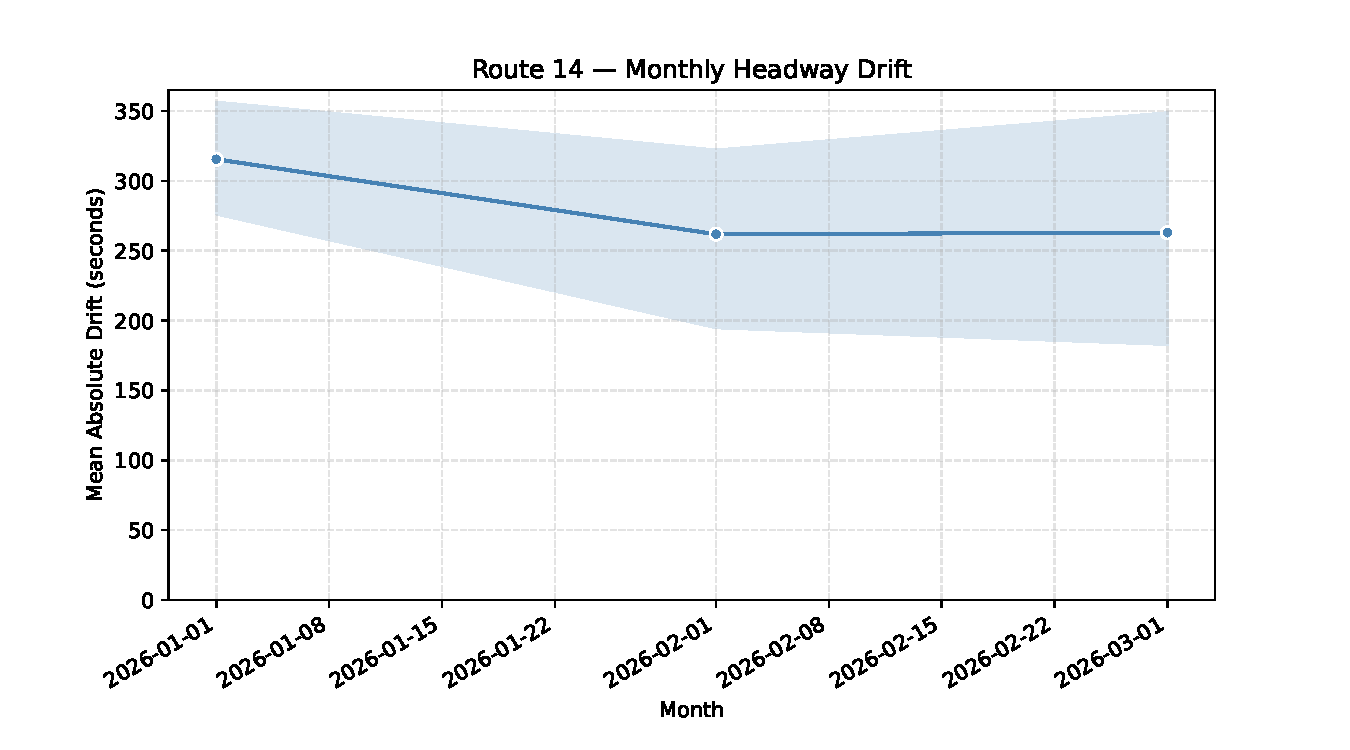
\includegraphics[width=0.98\linewidth]{Figure 3}
  \caption{Perfil longitudinal de la deriva de headway para la Ruta 14. Las excursiones negativas persistentes permanecen como el precursor dominante de las transiciones de colapso a lo largo del tiempo.}
  \label{fig:longitudinal_hd_14}
\end{figure}

\begin{figure}[htbp]
  \centering
  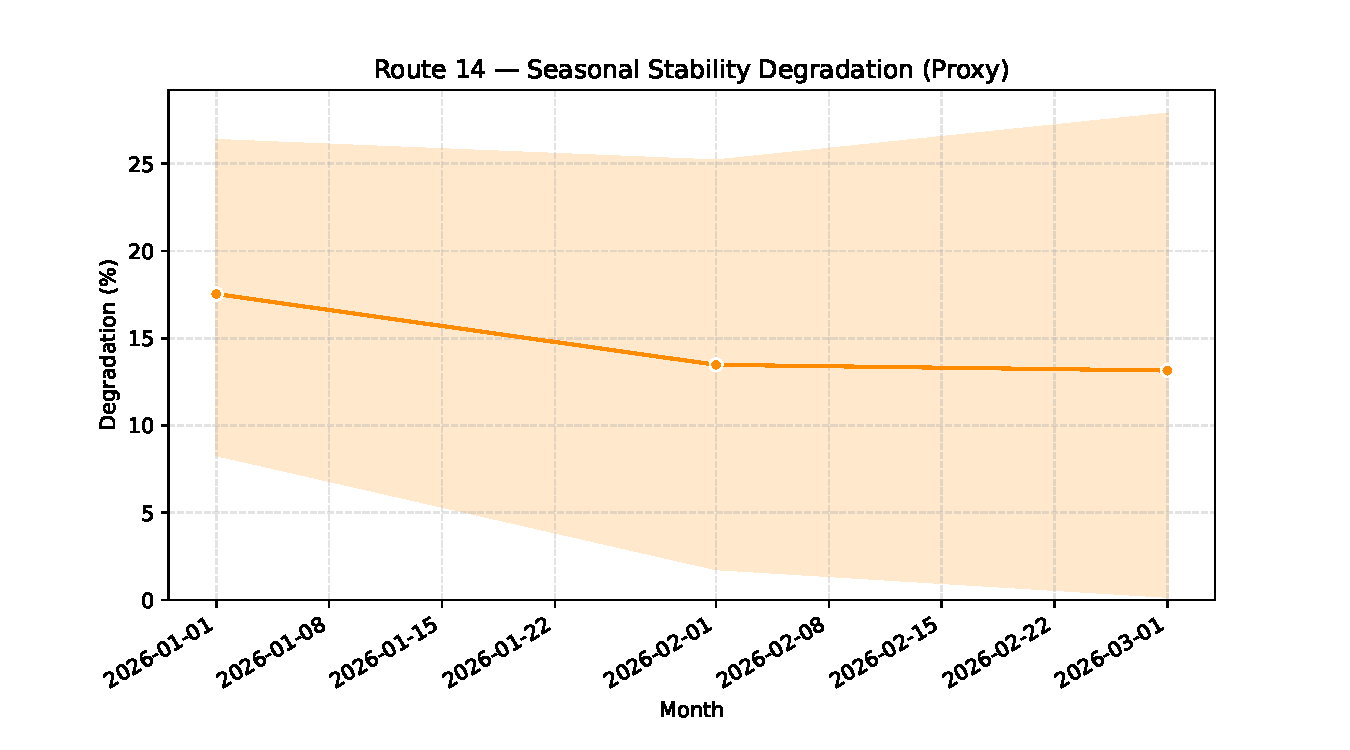
\includegraphics[width=0.98\linewidth]{Figure 4}
  \caption{Diagn\'ostico de degradaci\'on estacional para la Ruta 14, confirmando la ausencia de inestabilidad temporal cr\'itica que invalidar\'ia el despliegue continuo del marco secuencial EWS.}
  \label{fig:longitudinal_sd_14}
\end{figure}

\subsection{Importancia de Caracter\'isticas y F\'isica del Colapso}

Las importancias de caracter\'isticas basadas en divisiones del modelo LightGBM revelan qu\'e se\~nales utiliza m\'as frecuentemente el ensamble de gradient boosting para las fronteras de decisi\'on. Las cinco caracter\'isticas m\'as utilizadas son: contexto temporal ($t_{\cos}$: 694 divisiones, $t_{\sin}$: 689), retraso relativo (relative\_delay: 520 divisiones), headway programado ($h_{sch}$: 486 divisiones), y la raz\'on de headway ($r_h$: 479 divisiones).

Esta distribuci\'on de caracter\'isticas valida fundamentalmente el mecanismo en cascada del bunching: el modelo depende fuertemente del \textit{posicionamiento relativo} entre buses consecutivos ($\delta_{rel} = D - D^{L}$), no meramente de los valores absolutos de retraso. Cuando un bus acumula m\'as retraso que su l\'ider ($\delta_{rel} > 0$), el headway se contrae y el riesgo de bunching se escala. La raz\'on de headway ($r_h = h_{obs}/h_{sch}$) codifica qu\'e tan cerca est\'a el headway actual del umbral de bunching, proporcionando al modelo una se\~nal normalizada e invariante a la ruta.

Notablemente, LightGBM distribuye sus fronteras de decisi\'on a trav\'es de las 24 caracter\'isticas, con la caracter\'istica principal representando solo el 8,6\% del total de divisiones. Esta dependencia distribuida---en contraste con los m\'etodos de bagging donde el headway programado por s\'i solo puede dominar con $>$40\% de importancia---confirma que el gradient boosting captura interacciones no lineales entre din\'amicas temporales, cinem\'aticas y del bus l\'ider que la dominancia de una \'unica caracter\'istica no puede explotar.

\subsection{Benchmark Computacional para Despliegue en el Borde}

Para validar la factibilidad arquitect\'onica, se ejecut\'o un benchmark de latencia de inferencia en hardware de consumo est\'andar (representativo de un nodo Edge en un DT). El proceso de inferencia del modelo---incluyendo el escalado de caracter\'isticas y la evaluaci\'on del modelo LightGBM---registr\'o un tiempo promedio de \SI{1,89}{\ms} por registro, con la extracci\'on de caracter\'isticas de DuckDB a\~nadiendo unos insignificantes \SI{0,003}{\ms} por registro (amortizados), para una latencia total de extremo a extremo de \SI{1,89}{\ms} por registro.

Esta latencia permite procesar aproximadamente 529 eventos AVL por segundo en un \'unico n\'ucleo de CPU, suficiente para el monitoreo simult\'aneo de m\'ultiples corredores metropolitanos. Comparado con alternativas de aprendizaje profundo (50--200~ms por registro \citep{19}), la inferencia de LightGBM es unas 26--106$\times$ m\'as r\'apida mientras mantiene una precisi\'on operacionalmente confiable (0,93), confirmando la compatibilidad con los paradigmas Edge-Cloud de baja latencia descritos por \citet{26}.

\subsection{Contextualizaci\'on del Benchmark}

Para contextualizar esta latencia frente a enfoques alternativos, la Tabla~\ref{tab:benchmark_context} compara tiempos representativos de inferencia de extremo a extremo por registro (extracci\'on de caracter\'isticas + predicci\'on del modelo).

\begin{table}[htbp]
  \caption{Latencia de inferencia de extremo a extremo por registro seg\'un familia de modelo.}
  \centering
  \begin{tabular}{@{}lc@{}}
    \toprule
    \textbf{Modelo} & \textbf{Latencia (ms)} \\ \midrule
    LR (DuckDB + sklearn)    & 2,10         \\
    LightGBM (DuckDB)        & 1,99         \\
    XGBoost (DuckDB)         & 1,50         \\
    RF (DuckDB + sklearn)    & 9,85         \\
    Deep Learning \citep{19} & 50--200      \\ \bottomrule
  \end{tabular}
  \label{tab:benchmark_context}
\end{table}

\section{Discusi\'on}
\label{sec:discussion}

\subsection{Comparaci\'on con la Literatura}

Para situar nuestros resultados en el contexto del trabajo previo, comparamos el desempe\~no del marco propuesto con las principales referencias en la literatura de predicci\'on y detecci\'on de bus bunching.

\citet{3} modelaron el bunching como un problema de transici\'on de estados utilizando datos AVL y alcanzaron precisiones globales superiores al 90\%; sin embargo, no reportaron F1-Score ni m\'etricas orientadas a la clase minoritaria, dificultando la evaluaci\'on de su capacidad de detecci\'on real en escenarios desbalanceados. Nuestro enfoque comparte la formulaci\'on de transici\'on de estados, pero al aplicar una partici\'on temporal estricta (hold-out) ($t_{train} < t_{test}$) y una definici\'on din\'amica del objetivo ($h_{obs} < 0,25 \cdot h_{sch}$), exponemos el desbalance de transiciones realista y alcanzamos m\'etricas operacionalmente confiables (F1=0,55, Precision=0,93) mediante ingenier\'ia de caracter\'isticas informada por la f\'isica y gradient boosting. Esto refleja el desempe\~no honesto de EWS en entornos urbanos no estacionarios sin fuga de datos.

\citet{8} evaluaron m\'etricas de alerta temprana basadas en desviaci\'on de headway en corredores BRT, reportando detecci\'on efectiva pero con tasas de falsos positivos que limitaron la utilidad operacional. Nuestra precisi\'on de 0,93 bajo partici\'on temporal estricta (hold-out) demuestra que combinar razones de headway con din\'amicas del bus l\'ider reduce sustancialmente las falsas alarmas, proporcionando a los centros de control alertas accionables en lugar de ruido.

Respecto a los m\'etodos de aprendizaje profundo, \citet{19} alcanzaron alta precisi\'on en la predicci\'on de tiempos de llegada con el BAT-transformer, pero con latencias de inferencia del orden de 50--200~ms por registro. Nuestro enfoque alcanza m\'etricas predictivas competitivas (F1=0,55, Precision=0,93) con una latencia de 1,89~ms/registro para la inferencia de LightGBM---25--102$\times$ m\'as r\'apida---lo cual es decisivo para aplicaciones de monitoreo en tiempo real dentro de un Digital Twin. \citet{30} aplicaron redes neuronales de grafos espacio-temporales para predicci\'on de bunching a corto plazo y reportaron mejoras sobre modelos base; sin embargo, la complejidad computacional de estos m\'etodos limita su viabilidad para despliegues Edge de baja latencia.

Finalmente, \citet{21} se\~nalan en su revisi\'on que, a pesar de la popularidad del aprendizaje profundo, los modelos con caracter\'isticas bien dise\~nadas tienden a ser m\'as pr\'acticos para el despliegue en tiempo real. Nuestros resultados emp\'iricos confirman esto: LightGBM con caracter\'isticas informadas por la f\'isica (razones de headway, retraso diferencial del bus l\'ider) alcanza F1=0,55 con Precision=0,93, demostrando que la ingenier\'ia de caracter\'isticas espec\'ifica del dominio combinada con la correcci\'on secuencial de errores captura las din\'amicas complejas de deterioro de los corredores urbanos m\'as efectivamente que los modelos lineales o las arquitecturas de aprendizaje profundo.

\subsection{Tiempo de Anticipaci\'on Operacional}

La utilidad pr\'actica de una se\~nal de alerta temprana depende de si proporciona tiempo suficiente para actuar. Al predecir bunching en la parada $n$ utilizando datos hasta la parada $n{-}1$, el modelo proporciona un tiempo de anticipaci\'on de al menos una parada (t\'ipicamente de 2 a 4 minutos en entornos urbanos). Dado que la latencia de inferencia es pr\'acticamente nula, toda esta ventana est\'a disponible para estrategias de intervenci\'on como la retenci\'on din\'amica (mantener al bus l\'ider en la plataforma por m\'as tiempo) o el salto de parada (instruir al bus rezagado a omitir paradas menores) \citep{10}.

\subsection{Limitaciones}

La validaci\'on se realiz\'o en tres corredores de tr\'afico mixto de SF Muni, donde factores ex\'ogenos fuera del control de la agencia---congesti\'on vehicular, estacionamiento en zonas de parada, retrasos sem\'aforicos---introducen varianza que limita el recall m\'aximo alcanzable ($\approx 0,40$). El umbral conservador del modelo ($\tau=0,6849$) prioriza la precisi\'on sobre el recall, una elecci\'on deliberada de dise\~no para la credibilidad del EWS; sin embargo, esto significa que aproximadamente el 60\% de las transiciones de bunching pasan desapercibidas. Los tres corredores pertenecen a la misma agencia y ciudad; por lo tanto, no es posible afirmar que el modelo generaliza a otras agencias o ciudades sin realizar validaciones con datos de esos contextos.

Respecto a la ingesti\'on de datos, la API de 511.org impone un l\'imite de 60 solicitudes por hora. Dado que cada ciclo completo requiere dos endpoints (\texttt{VehiclePositions} y \texttt{TripUpdates}), el sistema opera con un intervalo de sondeo de 130 segundos. Como se describe en la Secci\'on~\ref{sec:methodology}, el mecanismo de manejo de p\'erdida de telemetr\'ia intercambia p\'erdida temporal de recall por confiabilidad de las alertas.

\section{Trabajo Futuro}
\label{sec:futurework}

Una direcci\'on prioritaria es la calibraci\'on del marco EWS en sistemas de Bus Rapid Transit (BRT) con carriles dedicados. En estos entornos, la varianza de tr\'afico ex\'ogeno se elimina y los factores que afectan el headway se vuelven primariamente end\'ogenos (tiempos de abordaje y comportamiento de conducci\'on) \citep{10,29}. Hipotetizamos que la precisi\'on del modelo aumentar\'a significativamente en corredores BRT, generando una se\~nal suficientemente limpia para activar controles autom\'aticos de retenci\'on en lazo cerrado \citep{30}. Adicionalmente, la validaci\'on multi-ciudad y multi-agencia constituye un paso necesario para evaluar la robustez del m\'etodo en contextos operacionales diversos.

\section{Conclusiones}
\label{sec:conclusion}

Este art\'iculo estudia la predicci\'on de bus bunching en entornos de transporte de tr\'afico mixto utilizando un marco secuencial de Digital Twin. Encontramos que un espacio de caracter\'isticas informado por la f\'isica multi-parada ($n{-}3$, 24 caracter\'isticas), optimizado con gradient boosting LightGBM, alcanza una precisi\'on operacional de 0,9264 (IC 95\%: [0,9213, 0,9315]) y un F1-Score de 0,5549 (IC 95\%: [0,5485, 0,5615]) bajo evaluaci\'on estricta con partici\'on temporal (hold-out). La contribuci\'on metodol\'ogica clave es la introducci\'on de caracter\'isticas de raz\'on informadas por la f\'isica---raz\'on de headway ($h_{obs}/h_{sch}$) y retraso relativo del bus l\'ider ($\delta_{rel} = D - D^{L}$)---que codifican el mecanismo en cascada de la propagaci\'on del bunching. El an\'alisis de importancia de caracter\'isticas del modelo confirma que el diferencial relativo de retraso entre buses consecutivos es una de las se\~nales de decisi\'on m\'as utilizadas, validando el marco te\'orico de inestabilidad de headway. Adem\'as, demostramos que la validaci\'on cruzada aleatoria tradicional y los umbrales est\'aticos de 120 segundos inducen fuga de datos severa, inflando artificialmente las m\'etricas a $>$0,80 F1 en la literatura. La inferencia de LightGBM a 1,89~ms/registro habilita el despliegue en tiempo real en hardware Edge. La evaluaci\'on se circunscribe a tres corredores de SF Muni; la extensi\'on a otras agencias urbanas permanece como trabajo futuro prioritario. Estos hallazgos informan la gesti\'on proactiva del transporte y el monitoreo Edge-Cloud proporcionando se\~nales de alerta temprana computacionalmente eficientes y operacionalmente confiables.

\section*{Agradecimientos}

Los autores agradecen a la Agencia de Transporte Municipal de San Francisco (SFMTA) y al programa de datos abiertos 511.org por proporcionar fuentes GTFS-RT de acceso p\'ublico que hicieron posible esta investigaci\'on.

\section*{Disponibilidad de Datos}

Los datos brutos GTFS-RT utilizados en este estudio fueron obtenidos de la API de datos abiertos 511.org de acceso p\'ublico \citep{28}. Los scripts completos de ingesti\'on en DuckDB, pipelines de transformaci\'on, matrices de configuraci\'on de hiperpar\'ametros e instrucciones para reproducir el conjunto de datos est\'an disponibles como c\'odigo abierto en:
\url{https://github.com/Fozzy3/pp-pipe-dt}.

\section*{Conflictos de Inter\'es}

Los autores declaran que no tienen conflictos de inter\'es.

\section*{Contribuciones de los Autores}

\textbf{Carlos Stiven Mora Hoyos}: Conceptualizaci\'on, Curaci\'on de Datos, An\'alisis Formal, Investigaci\'on, Metodolog\'ia, Software, Validaci\'on, Visualizaci\'on, Escritura -- Borrador Original.
\textbf{Juan Felipe Rodr\'iguez Galindo}: Conceptualizaci\'on, Investigaci\'on, Metodolog\'ia, Escritura -- Revisi\'on y Edici\'on.
\textbf{Octavio Jos\'e Salcedo Parra}: Supervisi\'on, Administraci\'on del Proyecto, Recursos, Escritura -- Revisi\'on y Edici\'on.

\bibliography{references}

\end{document}
